\documentclass[border=10pt]{standalone}
\usepackage{tikz}
\usetikzlibrary{positioning, fit, arrows.meta, backgrounds, calc, shapes.geometric, decorations.pathreplacing}

\definecolor{jaxblue}{HTML}{4A90D9}
\definecolor{cppred}{HTML}{D94A4A}
\definecolor{jsyellow}{HTML}{E8A838}
\definecolor{rlgreen}{HTML}{3DAA5C}
\definecolor{searchpurple}{HTML}{8B5CF6}
\definecolor{evogold}{HTML}{D4A017}
\definecolor{llmteal}{HTML}{2CAAA8}
\definecolor{jitbg}{HTML}{E8F0FE}
\definecolor{backendgray}{HTML}{F0F0F0}
\definecolor{dataorange}{HTML}{E07020}
\definecolor{validgreen}{HTML}{2E8B57}

\begin{document}
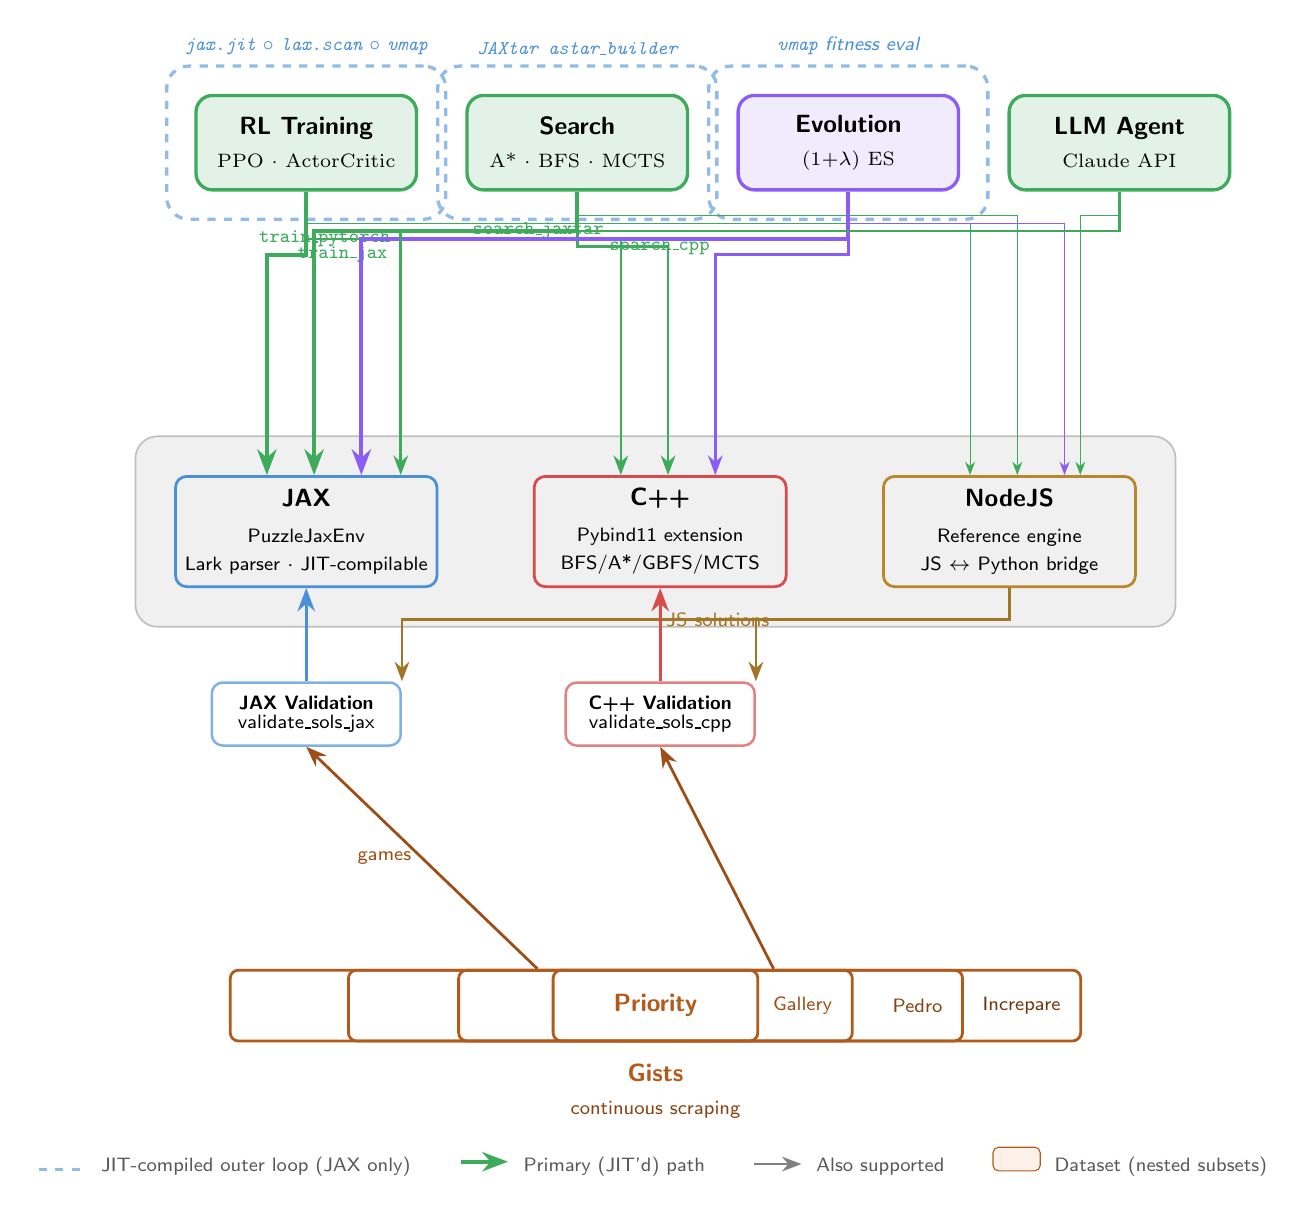
\begin{tikzpicture}[
    >=Stealth,
    node distance=0.8cm,
    backend/.style={
        draw, rounded corners=4pt, minimum width=3.2cm, minimum height=1.4cm,
        font=\sffamily\small, align=center, line width=1pt,
    },
    consumer/.style={
        draw, rounded corners=6pt, minimum width=2.8cm, minimum height=1.2cm,
        font=\sffamily\small\bfseries, align=center, line width=1.2pt,
    },
    dataset/.style={
        draw=dataorange!80!black, rounded corners=3pt, minimum height=0.9cm,
        font=\sffamily\small, align=center, line width=1pt,
    },
    validbox/.style={
        draw=validgreen!80!black, rounded corners=4pt, minimum width=2.4cm, minimum height=0.8cm,
        font=\sffamily\scriptsize, align=center, line width=0.9pt,
    },
    jitloop/.style={
        draw=jaxblue!60, dashed, rounded corners=8pt, line width=1.2pt,
        inner sep=8pt,
    },
    arrow/.style={->, line width=0.9pt, color=#1},
    labelstyle/.style={font=\sffamily\scriptsize, text=#1},
]

% ===== BACKENDS (middle) =====
\node[backend, draw=jaxblue] (jax) {
    \textbf{JAX}\\[2pt]
    \scriptsize PuzzleJaxEnv\\[-1pt]
    \scriptsize Lark parser $\cdot$ JIT-compilable
};

\node[backend, draw=cppred, right=1.2cm of jax] (cpp) {
    \textbf{C++}\\[2pt]
    \scriptsize Pybind11 extension\\[-1pt]
    \scriptsize BFS/A*/GBFS/MCTS
};

\node[backend, draw=jsyellow!80!black, right=1.2cm of cpp] (js) {
    \textbf{NodeJS}\\[2pt]
    \scriptsize Reference engine\\[-1pt]
    \scriptsize JS $\leftrightarrow$ Python bridge
};

% Backend abstraction box
\begin{scope}[on background layer]
\node[fit=(jax)(cpp)(js), fill=backendgray, rounded corners=8pt,
      inner xsep=14pt, inner ysep=14pt, draw=gray!50, line width=0.6pt] (backends) {};
\end{scope}

% ===== CONSUMERS (top) =====
\node[consumer, fill=rlgreen!15, draw=rlgreen, above=3.6cm of jax] (rl) {
    RL Training\\[1pt]
    \normalfont\scriptsize PPO $\cdot$ ActorCritic
};

\node[consumer, fill=rlgreen!15, draw=rlgreen, right=0.6cm of rl] (search) {
    Search\\[1pt]
    \normalfont\scriptsize A* $\cdot$ BFS $\cdot$ MCTS
};

\node[consumer, fill=searchpurple!12, draw=searchpurple, right=0.6cm of search] (evo) {
    Evolution\\[1pt]
    \normalfont\scriptsize $(1{+}\lambda)$ ES
};

\node[consumer, fill=rlgreen!15, draw=rlgreen, right=0.6cm of evo] (llm) {
    LLM Agent\\[1pt]
    \normalfont\scriptsize Claude API
};

% ===== JIT OUTER LOOPS =====
\node[jitloop, fit=(rl), inner sep=10pt, label={[labelstyle=jaxblue, font=\sffamily\scriptsize\itshape]above:{\texttt{jax.jit} $\circ$ \texttt{lax.scan} $\circ$ \texttt{vmap}}}] (jitrl) {};
\node[jitloop, fit=(search), inner sep=10pt, label={[labelstyle=jaxblue, font=\sffamily\scriptsize\itshape]above:{\texttt{JAXtar astar\_builder}}}] (jitsearch) {};
\node[jitloop, fit=(evo), inner sep=10pt, label={[labelstyle=jaxblue, font=\sffamily\scriptsize\itshape]above:{\texttt{vmap} fitness eval}}] (jitevo) {};

% ===== ARROWS: consumers -> backends =====
% RL
\draw[arrow=rlgreen, line width=1.4pt]
    (rl.south) -- ++(0, -0.8) -| ($(jax.north) + (-0.5, 0)$)
    node[pos=0.25, right, labelstyle=rlgreen] {\texttt{train\_jax}};
\draw[arrow=rlgreen]
    (rl.south) -- ++(0, -0.6) -| ($(cpp.north) + (-0.5, 0)$)
    node[pos=0.15, left, labelstyle=rlgreen] {\texttt{train\_pytorch}};
\draw[arrow=rlgreen, thin]
    (rl.south) -- ++(0, -0.4) -| ($(js.north) + (-0.5, 0)$);

% Search
\draw[arrow=rlgreen, line width=1.4pt]
    (search.south) -- ++(0, -0.5) -| ($(jax.north) + (0.1, 0)$)
    node[pos=0.22, right, labelstyle=rlgreen] {\texttt{search\_jaxtar}};
\draw[arrow=rlgreen]
    (search.south) -- ++(0, -0.7) -| ($(cpp.north) + (0.1, 0)$)
    node[pos=0.12, right, labelstyle=rlgreen] {\texttt{search\_cpp}};
\draw[arrow=rlgreen, thin]
    (search.south) -- ++(0, -0.3) -| ($(js.north) + (0.1, 0)$);

% Evolution
\draw[arrow=searchpurple, line width=1.4pt]
    (evo.south) -- ++(0, -0.6) -| ($(jax.north) + (0.7, 0)$);
\draw[arrow=searchpurple]
    (evo.south) -- ++(0, -0.8) -| ($(cpp.north) + (0.7, 0)$);
\draw[arrow=searchpurple, thin]
    (evo.south) -- ++(0, -0.4) -| ($(js.north) + (0.7, 0)$);

% LLM
\draw[arrow=rlgreen]
    (llm.south) -- ++(0, -0.5) -| ($(jax.north) + (1.2, 0)$);
\draw[arrow=rlgreen, thin]
    (llm.south) -- ++(0, -0.3) -| ($(js.north) + (0.9, 0)$);

% ===== VALIDATION LOOPS (between datasets and backends) =====
\node[validbox, draw=jaxblue!70] (vjax) at ($(jax.south) + (0, -1.6)$) {
    \textbf{JAX Validation}\\[-1pt]
    \scriptsize validate\_sols\_jax
};

\node[validbox, draw=cppred!70] (vcpp) at ($(cpp.south) + (0, -1.6)$) {
    \textbf{C++ Validation}\\[-1pt]
    \scriptsize validate\_sols\_cpp
};

% Arrows: NodeJS feeds into validation loops
\draw[arrow=jsyellow!70!black]
    (js.south) -- ++(0, -0.4) -| (vjax.north east)
    node[pos=0.3, right=4pt, labelstyle=jsyellow!70!black] {\scriptsize JS solutions};
\draw[arrow=jsyellow!70!black]
    (js.south) -- ++(0, -0.4) -| (vcpp.north east);

% Arrows: validation feeds back into JAX/C++ backends
\draw[arrow=jaxblue, line width=1.2pt]
    (vjax.north) -- (jax.south);
\draw[arrow=cppred, line width=1.2pt]
    (vcpp.north) -- (cpp.south);

% ===== DATASETS (bottom row) =====
% Nested subset structure: priority ⊂ gallery ⊂ pedro ⊂ increpare
\node[dataset, minimum width=10.8cm] (increpare) at ($(backends.south) + (0, -4.8)$) {};
\node[dataset, minimum width=7.8cm] (pedro) at (increpare.center) {};
\node[dataset, minimum width=5.0cm] (gallery) at (increpare.center) {};
\node[dataset, minimum width=2.6cm] (priority) at (increpare.center) {};

% Labels
\node[font=\sffamily\small\bfseries, text=dataorange!80!black] at (priority.center) {Priority};
\node[font=\sffamily\scriptsize, text=dataorange!70!black, anchor=east] at ($(gallery.east) + (-0.15, 0)$) {Gallery};
\node[font=\sffamily\scriptsize, text=dataorange!60!black, anchor=east] at ($(pedro.east) + (-0.15, 0)$) {Pedro};
\node[font=\sffamily\scriptsize, text=dataorange!50!black, anchor=east] at ($(increpare.east) + (-0.15, 0)$) {Increpare};

% Gists source
\node[font=\sffamily\small\bfseries, text=dataorange!80!black, anchor=north] at ($(increpare.south) + (0, -0.15)$) (gistlabel) {Gists};
\node[font=\sffamily\scriptsize, text=dataorange!60!black, anchor=north] at (gistlabel.south) {continuous scraping};

% Arrows: datasets feed up into validation loops
\draw[arrow=dataorange!70!black, line width=1.0pt]
    ($(increpare.north) + (-1.5, 0)$) -- (vjax.south)
    node[midway, left, labelstyle=dataorange!70!black] {games};
\draw[arrow=dataorange!70!black, line width=1.0pt]
    ($(increpare.north) + (1.5, 0)$) -- (vcpp.south);

% ===== LEGEND =====
\node[below=1.2cm of increpare, font=\sffamily\scriptsize, align=left, text=gray!70!black] (legend) {
    \tikz\draw[dashed, jaxblue!60, line width=1.2pt] (0,0) -- (0.6,0);
    \ JIT-compiled outer loop (JAX only) \qquad
    \tikz\draw[->, line width=1.4pt, rlgreen] (0,0) -- (0.6,0);
    \ Primary (JIT'd) path \qquad
    \tikz\draw[->, line width=0.9pt, gray] (0,0) -- (0.6,0);
    \ Also supported \qquad
    \tikz\node[draw=dataorange!80!black, fill=dataorange!10, rounded corners=2pt, minimum width=0.6cm, minimum height=0.3cm] {};
    \ Dataset (nested subsets)
};



\end{tikzpicture}
\end{document}
